%%%%%%%%%%%%%%%%%%%%%%%%%%%%%%%%%%%%%%%%%%%%%%%%%%%%%%%%%%
\begin{frame}[fragile] 
\frametitle{Spark Word Count: the driver}
%%%%%%%%%%%%%%%%%%%%%%%%%%%%%%%%%%%%%%%%%%%%%%%%%%%%%%%%%%
\begin{lstlisting}
	import org.apache.spark.SparkContext

	import org.apache.spark.SparkContext._

	val sc = new SparkContext("spark://...", "MyJob", "spark home", "additional jars") 
\end{lstlisting}

\begin{itemize}
	\item {\bf Driver and \texttt{SparkContext}}
	\begin{itemize}
		\item A SparkContext initializes the application driver, the latter then registers the application to the cluster manager, and gets a list of executors
		\item Then, the driver takes full control of the Spark job
	\end{itemize}
\end{itemize}

\end{frame}

%%%%%%%%%%%%%%%%%%%%%%%%%%%%%%%%%%%%%%%%%%%%%%%%%%%%%%%%%%
\begin{frame}[fragile] 
\frametitle{Spark Word Count: the code}
%%%%%%%%%%%%%%%%%%%%%%%%%%%%%%%%%%%%%%%%%%%%%%%%%%%%%%%%%%
\begin{lstlisting}
	val lines = sc.textFile("input")
	val words = lines.flatMap(_.split(" ")) 
	val ones = words.map(_ -> 1)
	val counts = ones.reduceByKey(_ + _) 
	val result = counts.collectAsMap()
\end{lstlisting}

\begin{itemize}
	\item {\bf RDD lineage DAG is built on driver side with}
	\begin{itemize}
		\item Data source RDD(s)
		\item Transformation RDD(s), which are created by transformations
	\end{itemize}

	\vspace{10pt}

	\item {\bf Job submission}
	\begin{itemize}
		\item An \emph{action} triggers the DAG scheduler to submit a job
	\end{itemize}
\end{itemize}

\end{frame}

%%%%%%%%%%%%%%%%%%%%%%%%%%%%%%%%%%%%%%%%%%%%%%%%%%%%%%%%%%
\frame {\frametitle{Spark Word Count: the DAG}
%%%%%%%%%%%%%%%%%%%%%%%%%%%%%%%%%%%%%%%%%%%%%%%%%%%%%%%%%%
\begin{figure}[h]
	\center
		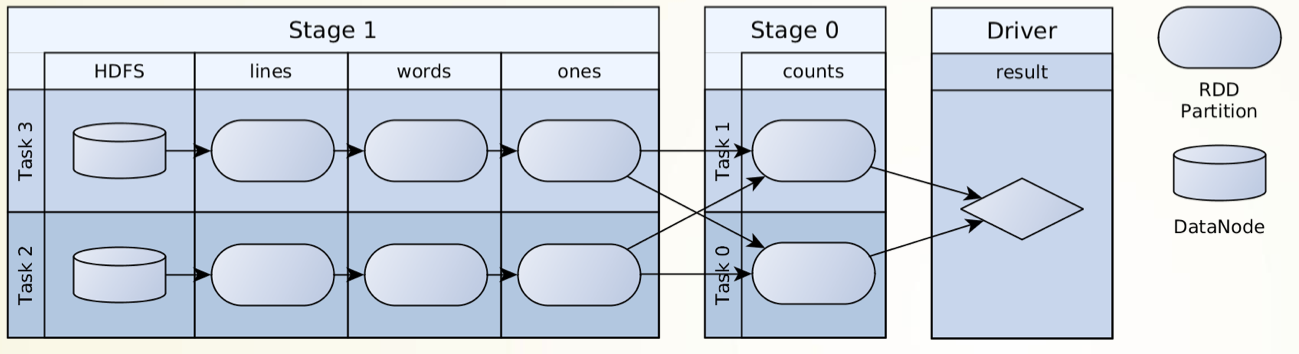
\includegraphics[scale=0.45]{./Figures/spark_wc_DAG}
\end{figure}

\begin{itemize}
	\item {\bf Directed Acyclic Graph}
	\begin{itemize}
		\item Built from the RDD lineage
	\end{itemize}

	\vspace{10pt}

	\item {\bf DAG scheduler}
	\begin{itemize}
		\item Transforms the DAG into stages and turns each partition of a stage into a single task
		\item Decides what to run
	\end{itemize}
\end{itemize}
}

%%%%%%%%%%%%%%%%%%%%%%%%%%%%%%%%%%%%%%%%%%%%%%%%%%%%%%%%%%
\frame {\frametitle{Spark Word Count: the execution plan}
%%%%%%%%%%%%%%%%%%%%%%%%%%%%%%%%%%%%%%%%%%%%%%%%%%%%%%%%%%
\begin{figure}[h]
	\center
		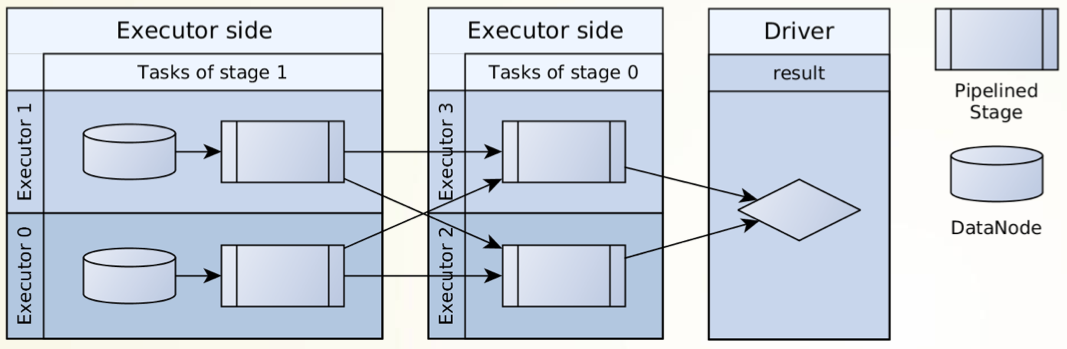
\includegraphics[scale=0.45]{./Figures/spark_wc_exec}
\end{figure}
\begin{itemize}
	\item {\bf Spark Tasks}
	\begin{itemize}
		\item Serialized RDD lineage DAG + closures of transformations
		\item Run by Spark executors
	\end{itemize}

	\vspace{20pt}

	\item {\bf Task scheduling}
	\begin{itemize}
		\item The driver side task scheduler launches tasks on executors according to resource and locality constraints
		\item The task scheduler decides where to run tasks
	\end{itemize}
\end{itemize}
}

%%%%%%%%%%%%%%%%%%%%%%%%%%%%%%%%%%%%%%%%%%%%%%%%%%%%%%%%%%
\begin{frame}[fragile] 
\frametitle{Spark Word Count: the Shuffle phase}
%%%%%%%%%%%%%%%%%%%%%%%%%%%%%%%%%%%%%%%%%%%%%%%%%%%%%%%%%%
\begin{lstlisting}
	val lines = sc.textFile("input")
	val words = lines.flatMap(_.split(" ")) 
	val ones = words.map(_ -> 1)
	val counts = ones.reduceByKey(_ + _) 
	val result = counts.collectAsMap()
\end{lstlisting}

\begin{itemize}
	\item {\bf reduceByKey transformation}
	\begin{itemize}
		\item Induces the shuffle phase
		\item In particular, we have a \emph{wide dependency}
		\item Like in Hadoop MapReduce, intermediate <key,value> pairs are stored on the local file system
	\end{itemize}

	\vspace{10pt}

	\item {\bf Automatic combiners!}
	\begin{itemize}
		\item The \texttt{reduceByKey} transformation implements map-side combiners to pre-aggregate data
	\end{itemize}
\end{itemize}

\end{frame}
